\documentclass[a4paper]{article}
\usepackage[utf8]{inputenc}
\usepackage{graphicx}
\usepackage[english]{babel}
\usepackage{amsmath}
\usepackage{amsthm}
\usepackage{multicol,caption}
\usepackage[T1]{fontenc}
\usepackage{listings}
\usepackage{color}

\theoremstyle{definition}
\newtheorem{definition}{Definition}[section]

\newenvironment{Figure}
{\par\medskip\noindent\center\minipage{0.9\linewidth}}
{\endminipage\par\bigskip\medskip}
  %figure inside multicols

\setlength{\oddsidemargin}{0pt}
% Marge gauche sur pages impaires
\setlength{\evensidemargin}{0pt}
% Marge gauche sur pages paires
\setlength{\textwidth}{450pt}
% Largeur de la zone de texte 
\setlength{\topmargin}{0pt}
% Pas de marge en haut
\setlength{\headheight}{13pt}
% Haut de page
\setlength{\headsep}{10pt}
% Entre le haut de page et le texte
\setlength{\footskip}{40pt}
% Bas de page + séparation
\setlength{\textheight}{633pt}
% Hauteur de la zone de texte 

%opening
\title{French Presidential Election Candidates Tweets}
\author{Nicolas Derumigny \and Emma Kerinec}

\begin{document}

\maketitle

\section{Introduction}
We have worked on a dataset of more than 3`000 tweets of the 11 French presidential election candidates posted during few years.
We have worked in Python 3 and used the following packages: Sklearn, Numpy, Matplotlib.

\section{Preprocessing}
We have chosen to keep only relevant words, in order to not give any power to a lot of very used words that do not bring any information (e.g. "le"). For that, we used a list of uninterested words (``stopwords''), improved with some specific words like ``https''.
We have also distinguish hashtags and other words as they do not have the same meaning in a tweet.
Because meaning of words is really context dependant and difficult to process we have choose to not consider semantic. 
 
\subsection{Simple Data}
Our first idea has been to compute frequencies of each word and each hashtag for each candidate.
We have seen that for a lot of candidates the few most frequent words confirm the view that people usually have about their opinions. 
We can see it with Philippe Poutou (cf images \ref{fig:image1}).


\begin{figure}
\begin{center}
\begin{multicols}{2}
\begin{tabular}{ | c | c |}
\hline Word & Frequency\\
\hline
contre & 1.25\%\\
gouvernement & 0.49\%\\
travail & 0.45\%\\
paris & 0.40\%\\
droite & 0.38\%\\
solidarité &  0.38\%\\
\hline
\end{tabular}

\begin{tabular}{ | c | c |}
\hline Hashtag & Frequency\\
\hline
\#npa & 11.03\%\\
\#loitravail & 2.98\%\\
\#grèce & 1.73\%\\
\#migrants & 1.66\%\\
\#poutou2017 & 1.45\%\\
\#hollande & 1.18\%\\
\hline
\end{tabular}
\end{multicols}
\bigskip
\captionof{figure}{\label{fig:image1} Most used words and hashtags for Phillipe Poutou}
\end{center}
\end{figure}

\section{Distance}
\theoremstyle{definition}
\begin{definition}{\bf Distance bewteen two sets of words:\\}
Measure the proportion of words that are different between two set of words $S_1$ and $S_2$:
\[
d(S_1, S_2)= \frac{1}{2} \cdot \Big( \sum_{\substack{w \in S_1\\w \notin S_2}}f(w) \quad + \quad \sum_{\substack{w \in S_2\\w \notin S_1}} f(w) \Big) 
\]
where $f(x)$ is the frequency of apparition of the word x.
\end{definition}

In that way we can compute the distance with respect to words and the distance with respect to hastags between two candidates.

\begin{figure}
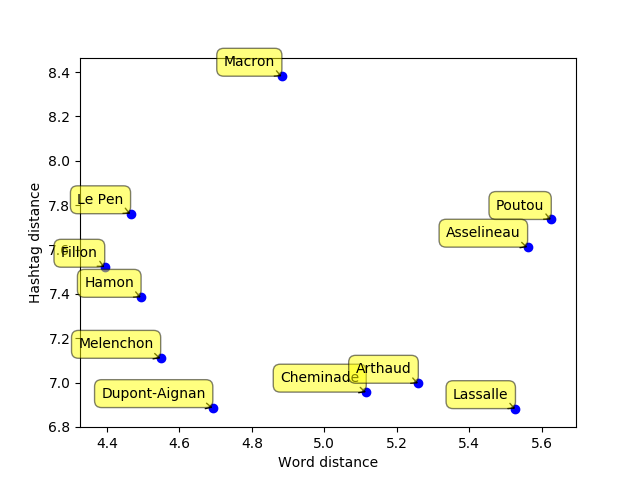
\includegraphics[width=\textwidth]{distances.png}
\captionof{figure}{\label{fig:image2} Sum of the distance to the other candidates, all words on $x$ and hashtags on $y$}
\end{figure}

It is interresting to see that Emmanuel Macron is the most different in hashtags and that Marine LePen et Jean-Luc Melechon often seen as extreme candidates are really common in the sense of the words they use (cf images \ref{fig:image2}).

\newpage
\section{Data Mining}
\subsection{Kmeans and Hierarchical clustering}
In order to partition candidates we have implemented k-means and Hierarchical clustering.
For two clusters on all tweets we obtain the same result with both methods (cf images \ref{fig:image3} and \ref{fig:image4}).


\begin{figure}
\begin{center}
\begin{multicols}{2}
\begin{tabular}{ | c | c |}
\hline
Poutou & Melenchon\\
Cheminade & Fillon\\
Arthaud & Hamon\\
Lassalle & Le Pen\\
Asselineau & Macron\\
& Dupont-Aignan\\
\hline
\end{tabular}
\captionof{figure}{\label{fig:image3} Words Similarities}
\bigskip

\begin{tabular}{ | c | c |}
\hline
Marcon & Melenchon\\
& Fillon\\
& Hamon\\
& Le Pen\\
& Dupont-Aignan\\
& Poutou\\
& Cheminade\\
& Arthaud \\
& Lassalle \\
& Asselineau \\
\hline
\end{tabular}
\bigskip
\captionof{figure}{\label{fig:image4} Hashtags Similarities}
\end{multicols}
\end{center}
\end{figure}

We can find that for the words there is a repartition minor/leading candidates and that for the hashtags Macron is alone (cf images \ref{fig:image3} and \ref{fig:image4}).

\subsection{Variation over time}
We have observed similar partitions for different periods, since our data cover a few years.

\begin{figure}
\begin{center}
\begin{multicols}{2}
\begin{tabular}{ | c | c |}
\hline
Melenchon & Fillon\\
Poutou & Le Pen\\
Cheminade & Macron\\
Hamon & Asselineau\\
Arthaud & Dupont-Aignan\\
Lassalle & \\
\hline
\end{tabular}
\captionof{figure}{\label{fig:image5} Hierarchical clustering on hashtags before the campaign}
\bigskip

\begin{tabular}{ | c | c |}
\hline
Melenchon & Poutou\\
Fillon & Cheminade\\
Hamon & Arthaud\\
Le Pen & Lassalle\\
Macron & Asselineau\\
& Dupont-Aignan\\
\hline
\end{tabular}
\bigskip
\captionof{figure}{\label{fig:image6} Hierarchical clustering on hashtags during the campaign}
\end{multicols}
\end{center}
\end{figure}

We can see that before the campaign the clustering is right/left candidates but during the campaign it is major/minor candidates (cf images \ref{fig:image5} and \ref{fig:image6}). We can observe this evolution during the campaign by divided it in some periods.


\subsection{A priori algorithm}
We have use the a priori algorithm in order to see the most frequent words associations for each candidate.

\begin{figure}
\begingroup
\fontsize{9pt}{12pt}
\texttt{ 
Melenchon\\
item: ('c',) , 0.120\\
Poutou\\
item: ('\#poutou2017',) , 0.140\\
item: ('c',) , 0.112\\
item: ('soir',) , 0.105\\
Fillon\\
item: ('fillon2017\_fr',) , 0.129\\
item: ('france',) , 0.114\\
item: ('francoisfillon',) , 0.184\\
item: ('veux',) , 0.105\\
Cheminade\\
item: ('\#cheminade2017',) , 0.422\\
item: ('\#cheminade2017', 'jcheminade') , 0.182\\
item: ('\#presidentielle2017',) , 0.137\\
item: ('jcheminade',) , 0.412\\
Hamon\\
item: ('veux',) , 0.101\\
Arthaud\\
item: ('c',) , 0.132\\
item: ('lutteouvriere',) , 0.112\\
item: ('lutteouvriere', 'n\_arthaud') , 0.102\\
item: ('n\_arthaud',) , 0.592\\
Le Pen\\
item: ('\#debattf1',) , 0.109\\
item: ('\#debattf1', '\#legranddebat') , 0.106\\
item: ('\#legranddebat',) , 0.108\\
item: ('france',) , 0.112\\
item: ('francais',) , 0.113\\
item: ('nos',) , 0.100\\
Macron\\
item: ('c',) , 0.123\\
Lassalle\\
item: ('\#presidentielle2017',) , 0.330\\
item: ('france',) , 0.106\\
item: ('jean',) , 0.109\\
item: ('jeanlassalle',) , 0.249\\
item: ('lassalle',) , 0.115\\
Asselineau\\
item: ('\#asselineau2017',) , 0.240\\
item: ('\#frexit',) , 0.229\\
item: ('\#frexit', '\#asselineau2017') , 0.161\\
item: ('\#presidentielle2017',) , 0.120\\
item: ('asselineau',) , 0.207\\
item: ('francois',) , 0.207\\
item: ('francois', 'asselineau') , 0.180\\
item: ('upr\_asselineau',) , 0.229\\
Dupont-Aignan\\
item: ('\#nda2017',) , 0.129\\
item: ('\#nda2017', 'dlf\_officiel') , 0.117\\
item: ('dlf\_officiel',) , 0.677\\
item: ('dupontaignan',) , 0.801\\
item: ('dupontaignan', '\#nda2017') , 0.121\\
item: ('dupontaignan', '\#nda2017', 'dlf\_officiel') , 0.116\\
item: ('dupontaignan', 'dlf\_officiel') , 0.660\\
item: ('dupontaignan', 'nicolas') , 0.145\\
item: ('dupontaignan', 'nicolas', 'dlf\_officiel') , 0.127\\
item: ('francais',) , 0.108\\
item: ('nicolas',) , 0.160\\
item: ('nicolas', 'dlf\_officiel') , 0.127\\
}
\endgroup
\captionof{figure}{\label{fig:image7}Use of the a priori algorithm}
\end{figure}

We have observed that the majority of the frequent itemsets are auto-citations: in politics, it seems to be more difficult to be known than well-known (cf figure \ref{fig:image7}).


\section{Observations}
We have been surprised that Emmanuel Macron who win the election extremely distinguish himself in the use of hashtags but not a lot in the use of words.
It has also been interesting to see that the distinction rigth/left is present during common periods but erase in favour of a partition minor/major candidates during the campaign.
It is important too to notice that the number of auto-citation and citation of other candidates is extremely important.
However, we have to deal the drawback of not using semantic indeed there is no link between different words with the same meaning, and even between singular and plural words.
We have also use the sklearn.feature\_extraction module in order to represent data as a sparse matrix of tokens. Sadly, we could only measure similarities between candidates without further explanation, as the original meaning of te tweet is lost.

\end{document}